\documentclass[t,xcolor=pdftex,dvipsnames,table]{beamer}
\usepackage[]{graphicx}\usepackage[]{color}
%% maxwidth is the original width if it is less than linewidth
%% otherwise use linewidth (to make sure the graphics do not exceed the margin)
\makeatletter
\def\maxwidth{ %
  \ifdim\Gin@nat@width>\linewidth
    \linewidth
  \else
    \Gin@nat@width
  \fi
}
\makeatother

\definecolor{fgcolor}{rgb}{0.345, 0.345, 0.345}
\newcommand{\hlnum}[1]{\textcolor[rgb]{0.686,0.059,0.569}{#1}}%
\newcommand{\hlstr}[1]{\textcolor[rgb]{0.192,0.494,0.8}{#1}}%
\newcommand{\hlcom}[1]{\textcolor[rgb]{0.678,0.584,0.686}{\textit{#1}}}%
\newcommand{\hlopt}[1]{\textcolor[rgb]{0,0,0}{#1}}%
\newcommand{\hlstd}[1]{\textcolor[rgb]{0.345,0.345,0.345}{#1}}%
\newcommand{\hlkwa}[1]{\textcolor[rgb]{0.161,0.373,0.58}{\textbf{#1}}}%
\newcommand{\hlkwb}[1]{\textcolor[rgb]{0.69,0.353,0.396}{#1}}%
\newcommand{\hlkwc}[1]{\textcolor[rgb]{0.333,0.667,0.333}{#1}}%
\newcommand{\hlkwd}[1]{\textcolor[rgb]{0.737,0.353,0.396}{\textbf{#1}}}%
\let\hlipl\hlkwb

\usepackage{framed}
\makeatletter
\newenvironment{kframe}{%
 \def\at@end@of@kframe{}%
 \ifinner\ifhmode%
  \def\at@end@of@kframe{\end{minipage}}%
  \begin{minipage}{\columnwidth}%
 \fi\fi%
 \def\FrameCommand##1{\hskip\@totalleftmargin \hskip-\fboxsep
 \colorbox{shadecolor}{##1}\hskip-\fboxsep
     % There is no \\@totalrightmargin, so:
     \hskip-\linewidth \hskip-\@totalleftmargin \hskip\columnwidth}%
 \MakeFramed {\advance\hsize-\width
   \@totalleftmargin\z@ \linewidth\hsize
   \@setminipage}}%
 {\par\unskip\endMakeFramed%
 \at@end@of@kframe}
\makeatother

\definecolor{shadecolor}{rgb}{.97, .97, .97}
\definecolor{messagecolor}{rgb}{0, 0, 0}
\definecolor{warningcolor}{rgb}{1, 0, 1}
\definecolor{errorcolor}{rgb}{1, 0, 0}
\newenvironment{knitrout}{}{} % an empty environment to be redefined in TeX

\usepackage{alltt}
\newcommand{\SweaveOpts}[1]{}  % do not interfere with LaTeX
\newcommand{\SweaveInput}[1]{} % because they are not real TeX commands
\newcommand{\Sexpr}[1]{}       % will only be parsed by R


%\documentclass[handout,t,xcolor=pdftex,dvipsnames,table]{beamer}  % For handout
\mode<presentation>{
\useoutertheme[subsection=false]{miniframes}
%\beamertemplatenavigationsymbolsempty
\usecolortheme{custom}
\usefonttheme[onlymath]{serif}
\setbeamercovered{invisible}
%\setbeamertemplate{navigation symbols}{}
%\setbeamertemplate{mini frames}{}  % Old one
% Comment out this line to give the header
% \setbeamertemplate{headline}[default]
\setbeamertemplate{caption}[numbered]
%\setbeamertemplate{itemize items}[circle] 
\setbeamertemplate{frametitle continuation}{\frametitle{\color{white}Title}}  % So no tile on subsequent frames, from [allowframebreaks]

%%% CUSTOMISING NAVIATION %%%%
%This customises the navigation to be thin width and just have section headings (not subsections). 
\setbeamertemplate{headline}{%
\leavevmode%
  \hbox{%
    \begin{beamercolorbox}[wd=\paperwidth,ht=2.5ex,dp=1.125ex]{palette tertiary}%   % Tertiary colour is blue
    \insertsectionnavigationhorizontal{\paperwidth}{}{\hskip0pt plus1filll}
    \end{beamercolorbox}%
}}}

\RequirePackage{marvosym}

%%% INCLUDING SOLUTIONS %%%%
%% You can incorporate both questions and solutions in the 
%% same document.  Solutions can be included between the 
%% commands \begin{soln} and \end{soln}
%% To generate a pdf with only the questions uncomment:
%\excludecomment{soln}
\usepackage{comment}
\specialcomment{soln}{\begingroup \vspace{1mm} \sl}{ \leavevmode \endgroup}

%%%% DETAILS FOR PART 1 TITLE PAGE (OLD) %%%%
%\title{\large Part2 - Probability \& Distribution Theory} 
%\subtitle{} 
%\author{\copyright Dr Di Warren 2016} 
%\date{MATH1005 - Statistics}
% \colorlet{Faculty}{Arts}
%\colorlet{Faculty}{MasterBrandRed} % This is only needed if the notes are used for different faculties.
%\colorlet{FacultyText}{White}
% Defines the color of the text used on the title page and ``blocks''
% White for Business; TitlePageBlack for Arts, Pharmacy and Science
%\definecolor{CoolBlack}{rgb}{0.0, 0.18, 0.39}

%%%% DETAILS FOR FULL COURSE TITLE PAGE %%%%
\title{\Huge STATISTICS} 
\subtitle{} 
\author{\copyright University of Sydney 2017 (Di Warren)} 
\date{MATH1005}
% \colorlet{Faculty}{Arts}
\colorlet{Faculty}{MasterBrandRed} % This is only needed if the notes are used for different faculties.
\colorlet{FacultyText}{White}
% Defines the color of the text used on the title page and ``blocks''
% White for Business; TitlePageBlack for Arts, Pharmacy and Science
\definecolor{CoolBlack}{rgb}{0.0, 0.18, 0.39}

%%%% PACKAGES %%%%
\usepackage{multirow}
\usepackage{fancybox}
\usepackage[english]{babel}
\usepackage[utf8]{inputenc}
\usepackage{bm}
\usepackage{array}
\usepackage{booktabs}
\usepackage{tikz}
\usetikzlibrary{matrix,arrows,decorations.pathmorphing}
\usepackage{verbatim}
\usepackage{pgf,pgfsys,pgffor}
\usepackage{pgfplots}
\pgfplotsset{compat=1.3} %Recommended as of Pgfplots 1.3 - necessary?
\usetikzlibrary{decorations.pathreplacing,calc}
\usetikzlibrary{shapes, backgrounds}   % For Venn diagrams
\def \setA{ (0,0) circle (1cm) }
\def \setB{ (1.5,0) circle (1cm) }
\def \setC{ (0.6,1.5) circle (1cm) }
\def \setO{ (-2, -1.5) rectangle (3.5, 2.75) }
\tikzstyle{every picture}+=[remember picture]
\tikzstyle{na} = [baseline=-.5ex]
\usepackage{listings}  %Added by Di for adding R code

%\AtBeginSection[]
%{
%   \begin{frame}
 %      \frametitle{Outline}
 %      \tableofcontents[currentsection]
%   \end{frame}
%}  %This seems overkill for weekly lecture slides.

%\AtBeginSection[]
%{
%  \begin{frame}
% \frametitle{Contents}
%  \tiny{\tableofcontents[currentsection]}
%  \end{frame}
%}
%\useoutertheme{infolines} % Just lists current section in navigation at top, nice but limiting?

%%%% TITLE PAGE AND CONTENTS AT BEGINNING OF EACH TOPIC %%%%

\RequirePackage{ifthen} % package required
\newboolean{sectiontoc}
\setboolean{sectiontoc}{true} %default to true

\AtBeginSection[]
{
\begin{frame}[plain]
\vspace{60pt}
\begin{center}
\Huge{{\textcolor{MasterBrandBlue} \insertsection}}
\end{center}
\begin{tikzpicture}[scale=0.54]
%\hspace{-12pt}
%% Big Rectangle
\fill[MasterBrandRed] (0,14) -- (20,14) -- (20,15) -- (0,15);

%\draw (1,14.5) node [anchor = west] {\textcolor{MasterBrandBlue}{\Huge{\insertsection}}}; Overlays box with title, but long titles drop off the page
\end{tikzpicture} 
\end{frame}

%%%%%WORKING VERSION OF TOC%%%%%
%\begin{frame}
%   \frametitle{Outline}
%  \tableofcontents[currentsection, sectionstyle=show/hide, subsectionstyle=show/show/hide]
%  \end{frame}
%}

%%%%%2 VERSIONS - WITH AND WITHOUT TOC%%%%%
  \ifthenelse{\boolean{sectiontoc}}{
    \begin{frame}
  \frametitle{Outline}
  \tableofcontents[currentsection, sectionstyle=show/hide, subsectionstyle=show/show/hide]
 \end{frame}
  }
}
%%%%%This doesnt seem to work?%%%%
\newcommand{\toclesssection}[1]{
  \setboolean{sectiontoc}{false}
  %\section{#1}
  \setboolean{sectiontoc}{true}
}


% PDF settings
%\hypersetup{%
%  pdftitle={\inserttitle \insertsubtitle},%
%  pdfauthor={Di Warren},%
%	pdfsubject={},%
%	pdfkeywords={}%   
%	 }

%%%%  HELPFUL MACROS %%%%
\newcommand{\ud}{\mathrm{d}}
\newcommand{\var}{\mathrm{var}}
\newcommand{\ep}{\varepsilon}
\newcommand{\cov}{\mathrm{cov}}
\newcommand{\tr}{\mathrm{tr}}
\newcommand{\MSE}{\mathrm{MSE}}
\newcommand{\rank}{\mathrm{rank}}
\newcommand{\Bias}{\mathrm{Bias}}
\newcommand{\dei}{\partial}
\newcommand{\E}{\mathbb{E}}
\newcommand{\N}{\mathcal{N}}
\newcommand{\bbR}{\mathbb{R}}
\newcommand{\V}{\mathbb{V}}
\newcommand{\betahat}{\hat{\beta}}
\newcommand{\CLRM}{$\mathbf{y} = X\bm{\beta} + \bm{\ep}$}

%%%% LOGO FOR SLIDES %%%%
\logo{\vspace{79mm}
\includegraphics[height=0.9cm]{../images/sydney.pdf}}

%%%% ADD PAGE NUMBER %%%%
\setbeamertemplate{sidebar right}{}
\setbeamertemplate{footline}{%
\hfill\usebeamertemplate***{navigation symbols}
\hspace{1cm}\insertframenumber{}/\inserttotalframenumber}

%%%% BEGIN CONTENT %%%


\begin{document}




%%%% TOPIC10 %%%%
\section[10]{Topic10: Test for Means (Z and T Tests)}

\subsection[Example1]{Example1: Comm Bank's online service}
\begin{frame}{Example1: Comm Bank's online service}

CommBank claims that an online personal loan application takes between 15-20 minutes to complete online.  There has been complaints that the applications take longer. A random sample of 26 customers results in the following data. 

{\tiny 
\begin{knitrout}
\definecolor{shadecolor}{rgb}{0.969, 0.969, 0.969}\color{fgcolor}\begin{kframe}
\begin{alltt}
\hlstd{x}\hlkwb{=}\hlkwd{c}\hlstd{(}\hlnum{29.3}\hlstd{,}\hlnum{23.1}\hlstd{,}\hlnum{18.5}\hlstd{,}\hlnum{23.8}\hlstd{,}\hlnum{24.8}\hlstd{,}\hlnum{23.8}\hlstd{,}\hlnum{22.5}\hlstd{,}\hlnum{26.3}\hlstd{,}\hlnum{20.8}\hlstd{,}\hlnum{21.1}\hlstd{,}\hlnum{21.4}\hlstd{,}\hlnum{24.0}\hlstd{,}\hlnum{22.0}\hlstd{,}\hlnum{28.2}\hlstd{,}\hlnum{27.3}\hlstd{,}\hlnum{19.4}\hlstd{,}\hlnum{20.1}\hlstd{,}\hlnum{26.4}\hlstd{,}\hlnum{24.4}\hlstd{,}
\hlnum{24.0}\hlstd{,}\hlnum{21.0}\hlstd{,}\hlnum{22.8}\hlstd{,}\hlnum{29.4}\hlstd{,}\hlnum{22.9}\hlstd{,}\hlnum{26.7}\hlstd{,}\hlnum{24.0}\hlstd{)}
\end{alltt}
\end{kframe}
\end{knitrout}
}

{\bf Would this evidence contradict the company's claim?}

\begin{center}
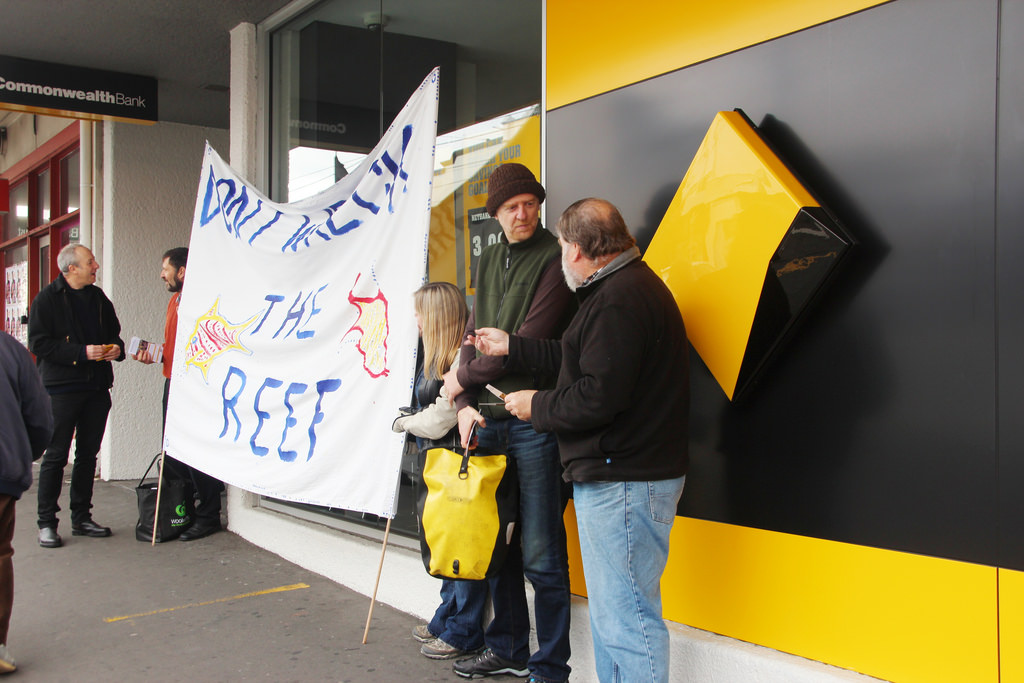
\includegraphics[height=3cm]{../images/CommBank.jpg}
\end{center}

\href{https://www.commbank.com.au/support/faqs/310.html}{\beamergotobutton{Comm Bank FAQ}}
\end{frame}


\subsection[Example2]{Example2: ADHD in children in Taiwan}
\begin{frame}{Example2: ADHD in children in Taiwan}

A study from 2013 looked at the long-term effects of stimulants on neurocognitive performance of Taiwanese children with attention deficit hyperactivity disorder (ADHD) using the Wechsler Intelligence Scale (WISC-III).  

\vspace{.5cm}
"In Taiwan, a high prevalence rate of ADHD was noticed about ten years ago, but there is still little research comparing neurocognitive function between children with ADHD and healthy children."  \\
"Due to the nature of the populations sampled, diagnostic criteria used, cultural differences, and methodological limitations, the prevalence of ADHD in various cultures varies. 
The prevalence is estimated to be about 8.4–11.7\% in Taiwan; 2.4\% in Australia; and 4\% in Japan."
\end{frame}


\begin{frame}{}

It was found that the 47 children in the control group (without ADHD) had a BMI (body mass index) of 18.8 with standard deviation 3.3, and the group of 171 children with ADHD had a BMI of 18.5 with standard deviation 3.7.

\vspace{.5cm}
{\bf Is there evidence that children with ADHD have a different BMI than the general population?}

\href{http://www.ncbi.nlm.nih.gov/pmc/articles/PMC4235029/}{\beamergotobutton{Abstract}}
\href{http://www.ncbi.nlm.nih.gov/pmc/articles/PMC4235029/table/T1/}{\beamergotobutton{TableT1}}
\href{http://www.ncbi.nlm.nih.gov/pmc/articles/PMC4235029/table/T2/}{\beamergotobutton{TableT2}}
\href{http://www.cdc.gov/healthyweight/assessing/bmi/childrens_bmi/about_childrens_bmi.html}{\beamergotobutton{BMI}}
\end{frame}


\subsection[Example3]{Example3: Weight Loss}
\begin{frame}{Example3: Weight Loss}

The amount of weight loss by a person taking a weight loss program depends on many factors, including gender, age, height, genetic background and fitness.   
To compare 2 programs, 20 people were ‘matched’ for gender/age/height. Each person in the pair was expected to act similarly to the other, but possibly quite differently to those in other pairs. This is called a ‘Case-Control’ study. 

\vspace{.5cm}
The weight losses (in kg) under the 2 programs A and B were as follows.

\vspace{.5cm}
{\small \begin{tabular}{lllllllllll} \hline
Pair & 1 & 2 & 3 & 4 & 5 & 6 & 7 & 8 & 9 & 10 \\ \hline
Diet $A$ & 3.6 & 1.1 & 6.2 & 11.3 & 0.5 & 8.5 & 12.4 & 2.5 & 4.1 & 6.2 \\
Diet $B$ & 3.2 & 0.7 & 7.1 & 9.8 & 1.1 & 7.1 & 11.5 & 2.5 & 2.9 & 5.0 \\  \hline
%$D = B-A$ & & & & & & & & & & \\ \hline
\end{tabular}}

\vspace{.5cm}
{\bf Is there a difference between the 2 diets?}
\end{frame}


\subsection[Z Test]{1 Sample Z Test}
\begin{frame}[fragile]{Steps for 1 Sample Z Test}

\framebox{Context}
Consider a population with unknown mean $\mu$ and known variance $\sigma^{2}$. We want to test a hypothesis about $\mu$.

\vspace{.5cm}
\framebox{H} $H_{0}: \mu = \mu_{0}$ vs $H_{1}: \mu < \mu_{0}$. 

\vspace{.5cm}
\framebox{A} The population variance $\sigma^{2}$ is known. The population is Normal or we have a large enough sample size $n$ to ensure Normality of $\bar{X}$ by the CLT.

\vspace{.5cm}
\framebox{T} 
\begin{itemize}
\item $\tau = Z = \frac{\bar{X} - \mu_{0}}{\frac{\sigma}{\sqrt{n}}}  \sim N(0,1)$ under $H_{0}$. 
\item Small values of $z$ will argue against $H_{0}$ for $H_{1}$. 
\item The observed value is $z$. 
\end{itemize}

\end{frame}  


\begin{frame}[fragile]{}

\framebox{P} $P$-value = $P( Z \leq z)$.

\vspace{.5cm}
\framebox{C} Weigh up the size of $P$-value.

\vspace{.5cm}
Notes on the Test Statistic and P-value.

\begin{itemize}
\item If the alternate hypotheses is $H_{1}: \mu > \mu_{0}$, then large values of $z$ will argue against $H_{0}$ for $H_{1}$ and the associated $P$-value is $P( Z \geq z)$. 
\item If the alternate hypotheses is 2 sided $H_{1}: \mu \neq \mu_{0}$, then both small and large values of $z$ will argue against $H_{0}$ for $H_{1}$ and the associated $P$-value is $2P( Z \geq z)$ due to symmetry.
\item We can also use the unstandardised random variable $\bar{X}$ as the test statistic, where $\bar{X} \sim N(\mu_{0}, \frac {\sigma^2}{n})$ under $H_{0}$.
\end{itemize}

\end{frame}  

\begin{frame}[fragile]{Example}

\begin{block}{CommBank}
Do CommBank online personal loan applications take longer than advertised?
\end{block}

\vspace{.5cm}
Let $\mu$ = Mean time for CommBank online personal loan application. Note this is a 1 sided test as we are testing whether the time is `longer'.

\vspace{.5cm}
\framebox{H} 
We will use the upper bound (most conservative) of the claim, so  
$H_{0}: \mu = 20$ vs $H_{1} = \mu > 20$.

\vspace{.5cm}
\framebox{A} The $n=26$ people in the  survey are sampled randomly. Here we do not have a given value of $\sigma$, but to illustrate the $Z$ test, we will choose $\sigma = 5$.
\end{frame}


\begin{frame}[fragile]{}

\framebox{T} 
\begin{itemize}
\item $\tau = Z = \frac{\bar{X} - \mu_{0}}{\frac{\sigma}{\sqrt{n}}}  \sim N(0,1)$ under $H_{0}$. 
\item Large values of $z$ will argue against $H_{0}$ for $H_{1}$. 
\item As $\bar{x}=23$ and we have assumed $\sigma=5$, the observed value is $z=  \frac{\bar{x} - \mu_{0}}{\frac{\sigma}{\sqrt{n}}} = \frac{23 - 20}{\frac{5}{\sqrt{26}}} \approx 3.06$.
\end{itemize}



\end{frame}  


\begin{frame}[fragile]{}
\framebox{P} $P$-value = $P( Z \geq 3.06) \approx  0.001$.

\begin{knitrout}
\definecolor{shadecolor}{rgb}{0.969, 0.969, 0.969}\color{fgcolor}\begin{kframe}
\begin{alltt}
\hlnum{1}\hlopt{-}\hlkwd{pnorm}\hlstd{(}\hlnum{3.06}\hlstd{)}
\end{alltt}
\begin{verbatim}
## [1] 0.001106685
\end{verbatim}
\begin{alltt}
\hlnum{1}\hlopt{-}\hlkwd{pnorm}\hlstd{(}\hlnum{23}\hlstd{,}\hlnum{20}\hlstd{,}\hlnum{5}\hlopt{/}\hlkwd{sqrt}\hlstd{(}\hlnum{26}\hlstd{))}
\end{alltt}
\begin{verbatim}
## [1] 0.001108861
\end{verbatim}
\end{kframe}
\end{knitrout}

\framebox{C} As the $P$-value is so small, we would question whether the claim is true.
\end{frame}  





\subsection[T Test]{1 Sample T Test}
\begin{frame}[fragile]{1 Sample T Test}

In some contexts, it is reasonable to assume that $\sigma^2$ is known, and the $Z$ Test hinges on this. But what happens when this assumption is not valid? 

\vspace{.5cm} Can we simply replace $\sigma$ (population) by $s$ (sample) in the $Z$ test? 
Can we change the Test Statistic from $\tau = \frac{\bar{X} - \mu_{0}}{\frac{\sigma}{\sqrt{n}}} \sim N(0,1)$ 
to $\tau = \frac{\bar{X} - \mu_{0}}{\frac{s}{\sqrt{n}}} \sim N(0,1)$?

\vspace{.5cm}
This is not appropriate because $S$ is itself a random variable, not a constant like $\sigma$.  Hence, we find that
$\tau = \frac{\bar{X} - \mu_{0}}{\frac{s}{\sqrt{n}}} \sim t_{n-1}$
which is a $t$ distribution with $n-1$ degrees of freedom. However, this also requires the extra assumption that the population is Normal.
\end{frame}

\begin{frame}[fragile]{Steps for the Student's T Test}

\framebox{Context}
Consider a population with unknown mean $\mu$ and unknown variance $\sigma^{2}$. We want to test a hypothesis about $\mu$.

\vspace{.5cm}
\framebox{H} $H_{0}: \mu = \mu_{0}$ vs $H_{1}: \mu < \mu_{0}$. \\

\framebox{A} The population is Normal. Check  this by a boxplot or histogram of the sample.

\framebox{T} 
\begin{itemize}
\item $\tau = T = \frac{\bar{X} - \mu_{0}}{\frac{s}{\sqrt{n}}}  \sim t_{n-1}$ (under $H_{0}$). 
\item Small values of $T$ will argue against $H_{0}$ for $H_{1}$. 
\item The observed value is $t$. 
\end{itemize}

\framebox{P} $P$-value = $P( t_{n-1} \leq t)$.

\framebox{C} Weigh up size of $P$-value.
\end{frame} 

\begin{frame}[fragile]{Example}

\begin{block}{CommBank}
Do CommBank online personal loan applications take longer than advertised?
\end{block}

\vspace{.5cm}
We now use the $T$ test. This is preferable as the previous usage of $Z$ test required assuming that $\sigma = 5$. However, here we don't know whether the distribution is Normal, so this is a untested assumption. From the sample of 26 application times $\{ 23.6, 26.7, 22.9, \ldots, 24.3\}$, we have $\bar{x} \approx 23.8$ and $s \approx 2.92$.
%% use x=rnorm(36,23,4) to generate some data.

{\tiny 
\begin{knitrout}
\definecolor{shadecolor}{rgb}{0.969, 0.969, 0.969}\color{fgcolor}\begin{kframe}
\begin{alltt}
\hlkwd{mean}\hlstd{(x)}
\end{alltt}
\begin{verbatim}
## [1] 23.76923
\end{verbatim}
\begin{alltt}
\hlkwd{sd}\hlstd{(x)}
\end{alltt}
\begin{verbatim}
## [1] 2.928176
\end{verbatim}
\end{kframe}
\end{knitrout}
}
\end{frame}


\begin{frame}[fragile]{}

\framebox{H} 
$H_{0}: \mu = 20$ vs $H_{1} = \mu > 20$.

\vspace{.5cm}
\framebox{A} We assume that the population of claim times is Normally distributed.

\begin{knitrout}
\definecolor{shadecolor}{rgb}{0.969, 0.969, 0.969}\color{fgcolor}\begin{kframe}
\begin{alltt}
\hlkwd{hist}\hlstd{(x,}\hlkwc{main}\hlstd{=}\hlstr{"Histogram of Claim Times"}\hlstd{)}
\end{alltt}
\end{kframe}
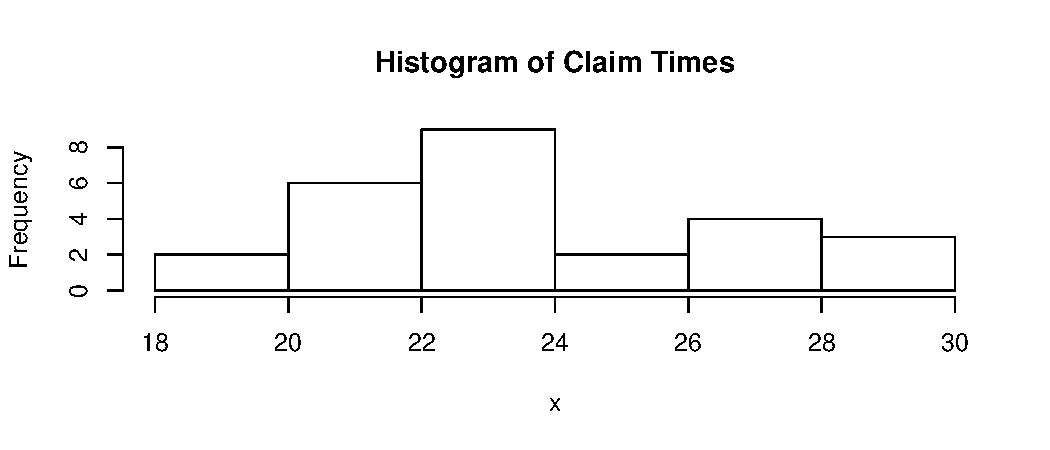
\includegraphics[width=\maxwidth]{figure/unnamed-chunk-6-1} 

\end{knitrout}
\end{frame}  

\begin{frame}[fragile]{}

\begin{knitrout}
\definecolor{shadecolor}{rgb}{0.969, 0.969, 0.969}\color{fgcolor}\begin{kframe}
\begin{alltt}
\hlkwd{boxplot}\hlstd{(x,}\hlkwc{horizontal}\hlstd{=T)}
\end{alltt}
\end{kframe}
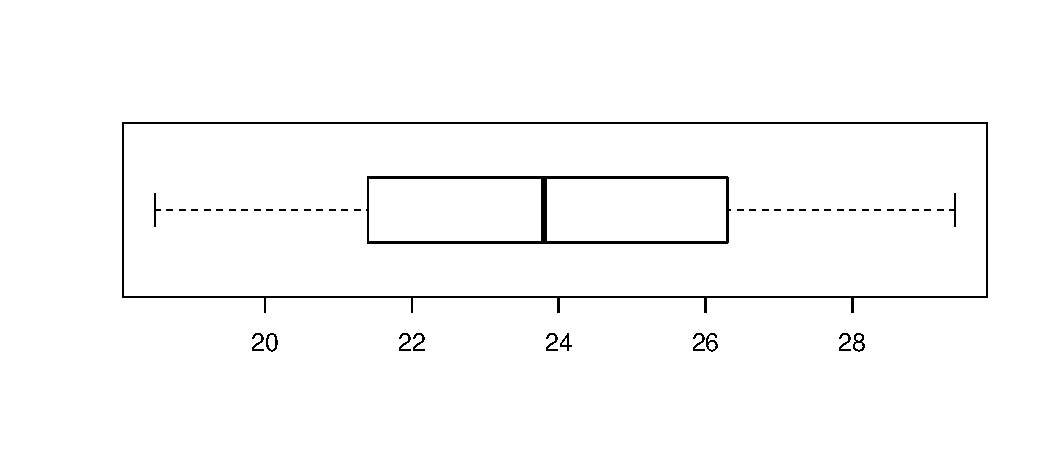
\includegraphics[width=\maxwidth]{figure/unnamed-chunk-7-1} 

\end{knitrout}
\end{frame}  






\begin{frame}[fragile]{}

\framebox{T} 
\begin{itemize}
\item $\tau = T = \frac{\bar{X} - \mu_{0}}{\frac{s}{\sqrt{n}}}  \sim t_{25}$ under $H_{0}$. 
\item Large values of $T$ will argue against $H_{0}$ for $H_{1}$. 
\item The observed value is $t=  \frac{\bar{x} - \mu_{0}}{\frac{s}{\sqrt{n}}} = \frac{23.8 - 20}{\frac{2.92}{\sqrt{26}}} \approx 6.64$
\end{itemize}

\framebox{P} $P$-value = $P( t_{25} \geq 6.64) \approx  0.0000007$.

\begin{knitrout}
\definecolor{shadecolor}{rgb}{0.969, 0.969, 0.969}\color{fgcolor}\begin{kframe}
\begin{alltt}
\hlnum{1}\hlopt{-}\hlkwd{pt}\hlstd{(}\hlnum{6.64}\hlstd{,}\hlnum{25}\hlstd{)}
\end{alltt}
\begin{verbatim}
## [1] 2.93773e-07
\end{verbatim}
\end{kframe}
\end{knitrout}

\vspace{.5cm}
\framebox{C} As the $P$-value is so small, again we question whether the claim is true.

\end{frame} 


\subsection[Paired T Test]{Paired T Test}
\begin{frame}[fragile]{Paired T Test}
The $T$ Test can also be applied to paired data. While the Sign Test only requires the population is continuous, the $T$ Test requires a stronger assumption: that the population of differences are Normal.

\vspace{.5cm}
\begin{block}{Sleep Study}
Is there a difference between the affect of drugs on sleep?
\end{block}
\end{frame}

\begin{frame}[fragile]{}
\begin{knitrout}
\definecolor{shadecolor}{rgb}{0.969, 0.969, 0.969}\color{fgcolor}\begin{kframe}
\begin{alltt}
\hlstd{a}\hlkwb{=}\hlkwd{c}\hlstd{(}\hlnum{0.7}\hlstd{,}\hlopt{-}\hlnum{1.6}\hlstd{,}\hlopt{-}\hlnum{0.2}\hlstd{,}\hlopt{-}\hlnum{1.2}\hlstd{,}\hlopt{-}\hlnum{0.1}\hlstd{,}\hlnum{3.4}\hlstd{,}\hlnum{3.7}\hlstd{,}\hlnum{0.8}\hlstd{,}\hlnum{0.0}\hlstd{,}\hlnum{2.0}\hlstd{)}
\hlstd{b}\hlkwb{=}\hlkwd{c}\hlstd{(}\hlnum{1.9}\hlstd{,}\hlnum{0.8}\hlstd{,}\hlnum{1.1}\hlstd{,}\hlnum{0.1}\hlstd{,}\hlopt{-}\hlnum{0.1}\hlstd{,}\hlnum{4.4}\hlstd{,}\hlnum{5.5}\hlstd{,}\hlnum{1.6}\hlstd{,}\hlnum{4.6}\hlstd{,}\hlnum{3.4}\hlstd{)}
\hlstd{diff}\hlkwb{=}\hlstd{b}\hlopt{-}\hlstd{a}
\hlkwd{mean}\hlstd{(diff)}
\end{alltt}
\begin{verbatim}
## [1] 1.58
\end{verbatim}
\begin{alltt}
\hlkwd{sd}\hlstd{(diff)}
\end{alltt}
\begin{verbatim}
## [1] 1.229995
\end{verbatim}
\begin{alltt}
\hlstd{tobs} \hlkwb{=} \hlstd{(}\hlkwd{mean}\hlstd{(diff)}\hlopt{-}\hlnum{0}\hlstd{)}\hlopt{/}\hlstd{(}\hlkwd{sd}\hlstd{(diff)}\hlopt{/}\hlkwd{sqrt}\hlstd{(}\hlnum{10}\hlstd{))}
\hlnum{2}\hlopt{*}\hlstd{(}\hlnum{1}\hlopt{-}\hlkwd{pt}\hlstd{(tobs,}\hlnum{9}\hlstd{))}
\end{alltt}
\begin{verbatim}
## [1] 0.00283289
\end{verbatim}
\end{kframe}
\end{knitrout}
\end{frame}


\begin{frame}[fragile]{}

\framebox{H}
$H_{0}: \mu = 0$ vs $H_{0}: \mu \neq 0$, where $\mu$ is the population mean of the differences $B-A$.

\vspace{.5cm}
\framebox{A} The set of differences is Normal.

\vspace{.5cm}
\begin{itemize}
\item $\tau = T = \frac{\bar{X} - \mu_{0}}{\frac{s}{\sqrt{n}}}  \sim t_{9}$ under $H_{0}$. 
\item Large and small values of $T$ will argue against $H_{0}$ for $H_{1}$. 
\item The observed value is $t=  \frac{\bar{x} - \mu_{0}}{\frac{s}{\sqrt{n}}} = \frac{1.58 - 0}{\frac{1.229995}{\sqrt{10}}} \approx 4.06$
\end{itemize}

\vspace{.5cm}
\framebox{P} $P$-value = $2 P( t_{9} \geq 4.06) \approx  0.003$.

\begin{knitrout}
\definecolor{shadecolor}{rgb}{0.969, 0.969, 0.969}\color{fgcolor}\begin{kframe}
\begin{alltt}
\hlnum{2}\hlopt{*}\hlstd{(}\hlnum{1}\hlopt{-}\hlkwd{pt}\hlstd{(}\hlnum{4.06}\hlstd{,}\hlnum{9}\hlstd{))}
\end{alltt}
\begin{verbatim}
## [1] 0.002841947
\end{verbatim}
\end{kframe}
\end{knitrout}

\vspace{.5cm}
\framebox{C} As the $P$-value is so small, again we would question whether the drugs are equivalent.
\end{frame}  





\subsection[T Test]{2 Sample T Test}
\begin{frame}[fragile]{2 Sample T Test}

The $T$ test (or $Z$ Test) can be generalised to cover 2 populations and samples as follows.

\vspace{.5cm}
\framebox{Context}
Consider 2 populations with unknown means $\mu_{X}$ and $\mu_{Y}$ and unknown common variance $\sigma^{2}$. We take 2 independent  samples. We want to test a hypothesis about $\mu_{X}-\mu_{Y}$.

\vspace{.5cm}
\framebox{H} $H_{0}: \mu_{X}-\mu_{Y} = c$ vs $H_{1}: \mu_{X}-\mu_{Y} < c$. (Note: Often $c = 0$.) \\

\vspace{.5cm}
\framebox{A} The 2 populations are  Normal with common $\sigma^2$. The 2 samples are independent.

\end{frame}  


\begin{frame}[fragile]{}

\framebox{T} 
\begin{itemize}
\item $\tau = T = \frac{ \bar{X} - \bar{Y} - c }{ s_{p}  \sqrt{ \frac{1}{n_{x}} + \frac{1}{n_{y}} }}  \sim t_{ n_{x} + n_{y}-2 }$ (under $H_{0}$),
where the pooled standard deviation is
$s_{p} = \sqrt{  \frac{ (n_{x}-1) s_{x}^2 +  (n_{y}-1) s_{y}^2 }{n_{x} + n_{y} -2}  }$.  
\item Small values of $T$ will argue against $H_{0}$ for $H_{1}$. 
\item The observed value is $t$. 
\end{itemize}

\vspace{.5cm}
\framebox{P} $P$-value = $P( t_{n_{x} + n_{y} -2} \leq t)$.

\vspace{.5cm}
\framebox{C} Weigh up size of $P$-value.
\end{frame}  


\begin{frame}[fragile]{Example}

\begin{block}{ADHD in children in Taiwan}
Is there evidence that children with ADHD have a different BMI to the general population?
\end{block}

\vspace{.5cm}
\framebox{Preparation}  \\
Let Population X = Control and Population Y = ADHD. \\
$\mu_{X}$ = Mean BMI of children in general population and $\mu_{Y}$= Mean BMI of children with ADHD. \\
$n_{x} = 47$, $\bar{x} = 18.8$, $s_{x} = 3.3$, $n_{y} = 171$, $\bar{y} = 18.5$, $s_{y} = 3.7$. \\
So $s_{p} = \sqrt{  \frac{ (n_{x}-1) s_{x}^2 +  (n_{y}-1) s_{y}^2 }{n_{x} + n_{y} -2}  } = 3.618522$.

\end{frame}



\begin{frame}[fragile]{}

\begin{knitrout}
\definecolor{shadecolor}{rgb}{0.969, 0.969, 0.969}\color{fgcolor}\begin{kframe}
\begin{alltt}
\hlstd{n_x}\hlkwb{=} \hlnum{47}
\hlstd{xbar}\hlkwb{=}\hlnum{18.8}
\hlstd{s_x}\hlkwb{=}\hlnum{3.3}
\hlstd{n_y}\hlkwb{=}\hlnum{171}
\hlstd{ybar}\hlkwb{=}\hlnum{18.5}
\hlstd{s_y}\hlkwb{=}\hlnum{3.7}
\hlstd{sp} \hlkwb{=} \hlkwd{sqrt}\hlstd{( ((n_x}\hlopt{-}\hlnum{1}\hlstd{)}\hlopt{*}\hlstd{s_x}\hlopt{^}\hlnum{2} \hlopt{+} \hlstd{(n_y}\hlopt{-}\hlnum{1}\hlstd{)}\hlopt{*}\hlstd{s_y}\hlopt{^}\hlnum{2}\hlstd{)}\hlopt{/}\hlstd{(n_x}\hlopt{+}\hlstd{n_y}\hlopt{-}\hlnum{2}\hlstd{) )}
\hlstd{sp}
\end{alltt}
\begin{verbatim}
## [1] 3.618522
\end{verbatim}
\begin{alltt}
\hlstd{t} \hlkwb{=} \hlstd{(xbar}\hlopt{-}\hlstd{ybar)}\hlopt{/}\hlstd{(sp}\hlopt{*}\hlkwd{sqrt}\hlstd{(}\hlnum{1}\hlopt{/}\hlstd{n_x} \hlopt{+} \hlnum{1}\hlopt{/}\hlstd{n_y))}
\hlstd{t}
\end{alltt}
\begin{verbatim}
## [1] 0.5033948
\end{verbatim}
\end{kframe}
\end{knitrout}
\end{frame}  

\begin{frame}[fragile]{}
\framebox{H} 
$H_{0}: \mu_{X} - \mu_{Y} = 0$ vs $H_{1} =  \mu_{X} - \mu_{Y} \neq  0$.

\vspace{.5cm}
\framebox{A} We assume that both population are Normally distributed with common variance, and that the 2 samples are independent. We do not have the raw data to be able to do histograms as a diagnostic.

\framebox{T} 
\begin{itemize}
\item $\tau = T = \frac{ \bar{X} - \bar{Y} - c }{ s_{p}  \sqrt{ \frac{1}{n_{x}} + \frac{1}{n_{y}} }}  \sim t_{ n_{x} + n_{y}-2 } \sim t_{47+171-2} = t_{216}$ under $H_{0}$. 
\item Large and small values of $T$ will argue against $H_{0}$ for $H_{1}$. 
\item The observed value is $t=  0.5033948$
\end{itemize}

\vspace{.5cm}
\framebox{P} $P$-value = $2 P( t_{216} \geq 0.5033948) \approx  0.615$.

\begin{knitrout}
\definecolor{shadecolor}{rgb}{0.969, 0.969, 0.969}\color{fgcolor}\begin{kframe}
\begin{alltt}
\hlnum{2}\hlopt{*}\hlstd{(}\hlnum{1}\hlopt{-}\hlkwd{pt}\hlstd{(}\hlnum{0.5033948}\hlstd{,}\hlnum{216}\hlstd{))}
\end{alltt}
\begin{verbatim}
## [1] 0.6151997
\end{verbatim}
\end{kframe}
\end{knitrout}
\end{frame}  

\begin{frame}[fragile]{}
\framebox{C} As the $P$-value is so big, there does not appear to be a difference in the BMIs of children with and without ADHD.
\end{frame} 

\begin{frame}{Why do we use the pooled variance? }

As with the 1 sample t test, we need an estimate of the unknown variance $\sigma^2$ (here by assumption, common for both populations). \\

Options for the estimate include:

\begin{itemize}
\item The sample variance of Population $X$: $s_{x}^2$.
\item The sample variance of Population $Y$: $s_{y}^2$.
\item The average of the sample variances: $\frac{s_{x}^2 + s_{y}^2}{2}$.
\item The weighted average of the sample variances: $s_{p}^2$. This takes into account both sample variances and the size of the samples. $s_{p}^2$ is always between $s_{x}^2$ and $s_{y}^2$.
\end{itemize}





\end{frame}





\begin{frame}{Summary: What do we do with 2 samples? }

We need to distinguish between a 1 sample test on differences (for paired data) and a 2 sample test on independent data. It is easy to make a mistake with wrong type of analysis. So we ask 2 critical questions:

\vspace{.5cm}
Q1: Are the 2 samples paired? Leads to 1 sample test of differences. \\
\vspace{.5cm}

Q2: Are the 2 samples independent? Leads to the 2 sample test.

\vspace{.5cm}
ANOVA (Not examinable) \\
We can extend this theory to 3 or more populations and samples. This is very useful in many research contexts, and is called Analysis of Variance.
\end{frame}




\end{document}
